\documentclass[a4paper]{article}
\usepackage[utf8]{inputenc}
\usepackage[unicode, colorlinks = true, linkcolor=black]{hyperref}
\usepackage{graphicx}
\usepackage[T1]{fontenc}
\usepackage[slovak]{babel}
\usepackage[margin=2cm]{geometry}
\usepackage{csquotes}
\usepackage{xcolor}
\usepackage{subfigure}

% appendix
\makeatletter
\g@addto@macro\appendix{%
  \cleardoublepage
  \section*{Přílohy}
  \addtocontents{toc}{\protect\contentsline{section}{Přílohy}{}{}}%
}
\makeatother

\begin{document}

\begin{titlepage}
\begin{center}
    \Huge
    \textsc{Vysoké učení technické v Brně\\[-0.2em]
    \huge
    Fakulta informačních technologií}\\
    \vspace{\stretch{0.382}}
    \large
    Mikroprocesorové a vestavěné systémy\\
    \LARGE
    Spínání světla dle intenzity\\
    \vspace{\stretch{0.618}}
    \Large
    \today \hfill Adam Zvara (xzvara01)
\end{center}
\end{titlepage}

\section{Úvod}

Cieľom tohto projektu je návrh a implementácia vstavanej aplikácie na doske WeMos D1 R32 UNO ESP32\footnote{\href{https://www.laskakit.cz/wemos-d1-r32-uno-esp32/}{https://www.laskakit.cz/wemos-d1-r32-uno-esp32/}}, ktorá realizuje spínanie LED podľa nameranej intenzity osvetlenia zo senzoru BH1750\footnote{\href{https://www.laskakit.cz/snimac-intenzity-osvetleni-bh1750/}{https://www.laskakit.cz/snimac-intenzity-osvetleni-bh1750/}}.
Okrem dosky a senzoru systém obsahuje 2 LED diódy, ktorých jas je dynamicky nastaviteľný počas behu aplikácie. Na základe nameranej intenzity je ovládaný jas prvej diódy a pomocou sériovej komunikácie je možné zadať prahovú intenzitu, pri ktorej dôjde ku aktivácií druhej diódy.

Program je napísaný v jazyku C s použitím frameworku ESP-IDF\footnote{\href{https://github.com/espressif/esp-idf}{https://github.com/espressif/esp-idf}} a vývojového prostredia PlatformIO\footnote{\href{https://platformio.org/}{https://platformio.org/}}.

\section{Zapojenie hardware}
Senzor a diódy sú na dosku pripojené externe na nepájavom poli a to následujúcim spôsobom.

\subsection*{Senzor BH1750}
Senzor realizuje meranie svetelnej intenzity a pomocou sériovej zbernice I2C \cite{I2Cdoc} a obsahuje 5 vývodov:
\begin{itemize}
    \item Napájanie (3.3V) -- napojený na ESP32 pin \textbf{3V3}
    \item Uzemnenie -- napojený na jeden z ESP32 pinov \textbf{GND}
    \item SCL (Serial clock) -- napojený na ESP32 pin \textbf{SCL}
    \item SDA (Serial data) -- napojený na ESP32 pin \textbf{SDA}
    \item ADDR -- nastavuje adresu senzoru (ak je odpojený alebo pripojený na zem, adresa je 0x23)
\end{itemize}

\subsection*{LED}
LED svetlá sú zapojené na \textbf{GPIO} piny \textbf{25} a \textbf{26}. Medzi LED svetlami a zdrojom sú napojené rezistory s veľkosťou 330$\Omega$, aby došlo ku zmenšeniu prúdu prechádzajúceho LEDkami a nezničili sa.

\subsection*{Celkové zapojenie}
Výsledné zapojenie je možné sledovať na nasledujúcich obrázkoch.

\begin{figure}[h]
    \centering
    \subfigure{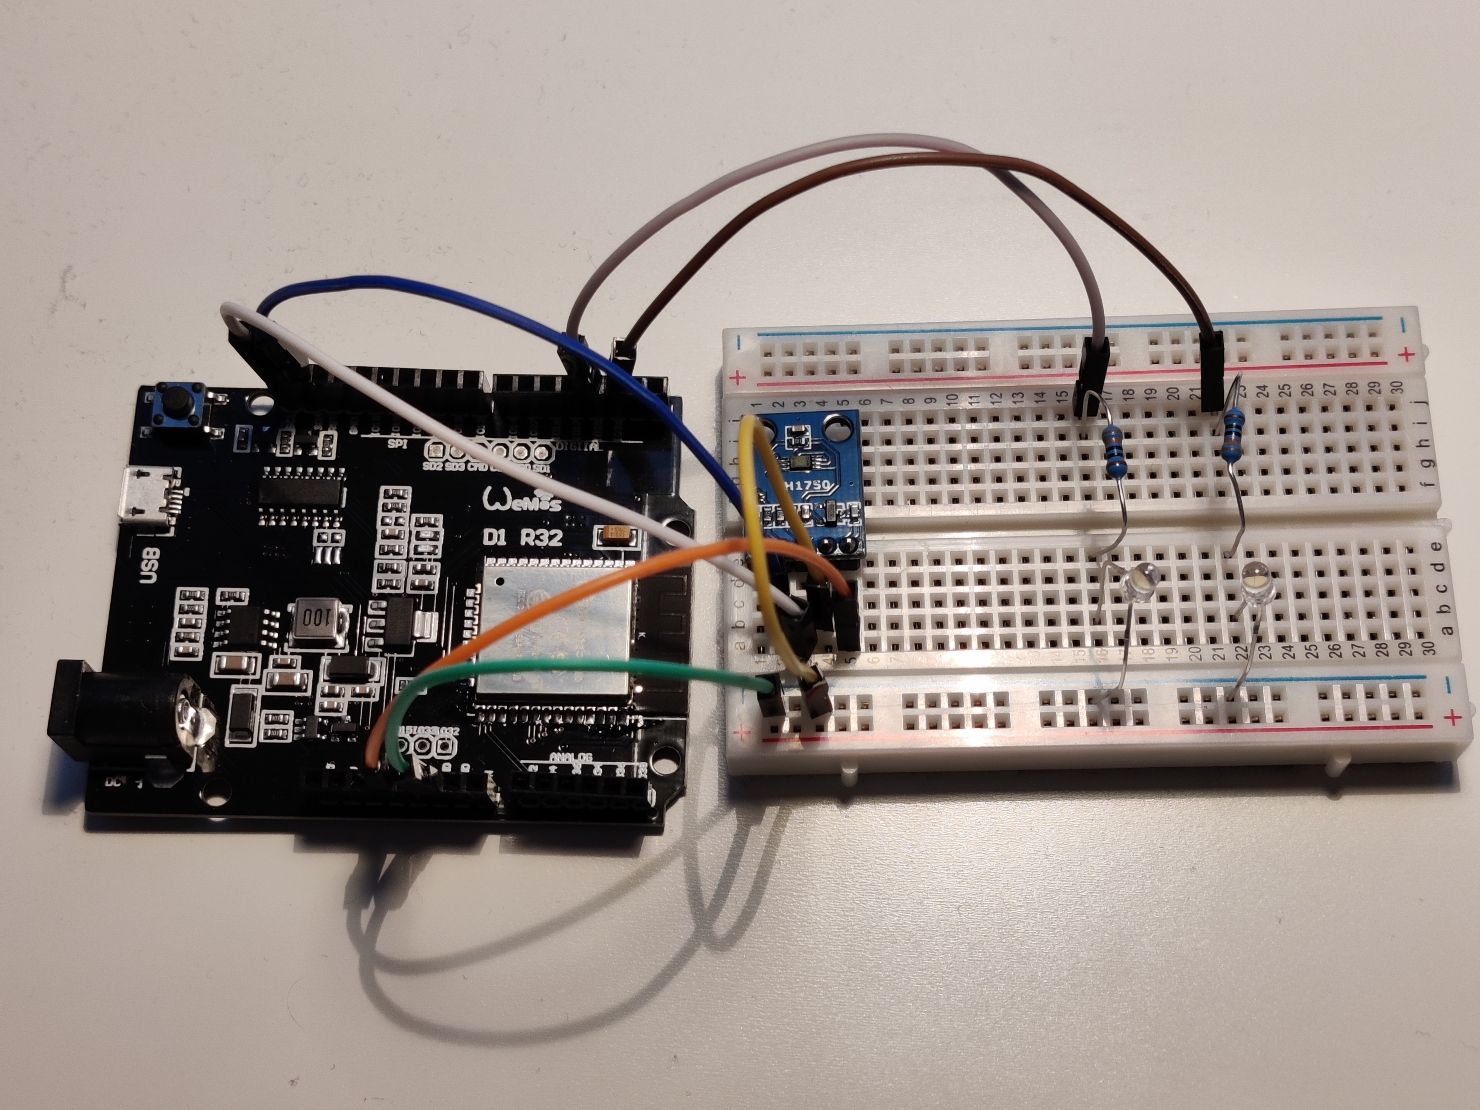
\includegraphics[scale=0.15]{img/board.jpg}}
    \hfill
    \subfigure{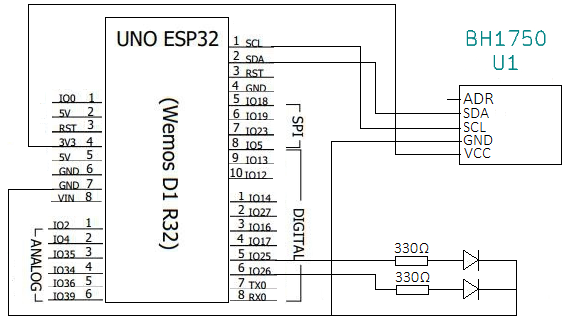
\includegraphics[scale=0.9]{img/scheme.png}}
    \caption{Fyzické zapojenie (a) a schéma zapojenia (b)}
    \label{zapojenie}
\end{figure}

\newpage
\section{Popis riešenia}
Táto sekcia popisuje programové riešenie spolu s využitými modulmi ESP32 a dekompozíciou úlohy na pod-problémy. Implementácia je v jednom súbore \textbf{main.c}, ktorý sa nachádza v zložke \texttt{src}. 
Ostatné súbory boli vygenerované prostredím PlatformIO. Pri implementácií som vychádzal z dokumentácie ESP-IDF\footnote{\href{https://docs.espressif.com/projects/esp-idf/en/latest/esp32/index.html}{https://docs.espressif.com/projects/esp-idf/en/latest/esp32/index.html}} a vzorových príkladov použitia modulov\footnote{\href{https://github.com/espressif/esp-idf/tree/master/examples}{https://github.com/espressif/esp-idf/tree/master/examples}}.

\subsection{Konfigurácia senzoru}
Pre spustenie činnosti senzoru je potrebné senzor po zapojení nakonfigurovať. Podľa dokumentácie \cite[str. 4]{sensordoc} je nutné poslať senzoru konfiguračnú správu, ktorou vyberieme
jeden z modov snímania \cite[str. 5]{sensordoc}. Od modu snímania závisí presnosť meraní a doba, po ktorej je možné dáta zo senzoru prečítať. V implementácií je použitý mód \texttt{Continuously H-Resolution Mode}. Módy je možné meniť nastavením parametru \textbf{BH1750\_SENZOR\_RES}. 

\subsection{Čítanie dát zo senzoru}
Po konfigurácií senzoru je možné pomocou I2C modulu\cite{I2Cdoc} získavať dáta o aktuálnej intenzite osvetlenia. Tento modul je taktiež nutné nakonfigurovať (funkcia \texttt{i2c\_master\_init}) a 
pomocou funkcie \texttt{master\_read\_slave} je možné načítavať dáta zo senzoru. Dáta sú predávané v poli s veľkosťou 2, pretože senzor najprv odošle vrchnú časť 16 bitového čísla a po nej spodných 8 
bitov. Nakoniec je z tohto poľa vytvorené jedno 16 bitové číslo, ktoré reprezentuje intenzitu osvetlenia v miestnosti. Pred jej použitím je nutné číslo \textbf{vydeliť hodnotou 1.2}\\\cite[str. 7]{sensordoc}.

\subsection{Načítavanie vstupu od užívateľa}
Komunikácia s užívateľom prebieha pomocou modulu UART \cite{UARTdoc}. Doska ESP32 obsahuje USB-to-UART most, pomocou ktorého je možné priamo z USB pripojenia zadávať konfiguráciu parametrov programu.
Pri nastavení modulu UART je potrebné zadať piny Rx a Tx, ktoré su pre pripojenie cez USB \textbf{GPIO 1} a \textbf{GPIO 3}\footnote{\href{https://www.esp32.com/viewtopic.php?t=13145}{https://www.esp32.com/viewtopic.php?t=13145}}.

\subsection{Ukladanie parametrov od užívateľa}
Užívateľ môže zadávať prahovú intenzitu, pri ktorej dôjde ku aktivovaniu druhej LEDky. Z požiadaviek zadania je nutné, aby táto hodnota ostala v pamäti aj po odpojení dosky od zdroju.
Na to slúži modul \textbf{NVS} \cite{NVSdoc}.

\subsection{Intenzita LED}
Poslednou časťou je ovládanie samotných LEDiek. Na nastavenie intenzity žiaru LED svetiel je použitý modul LEDC \cite{LEDCdoc}, ktorý generuje PWM signál, ktorým sa táto intenzita nastavuje.
Pomocou funkcie \texttt{set\_led} je možné nastavovať príslušnej LEDke \textbf{striedu}. Okrem toho je nutné sa zamyslieť nad mapovaním intervalu hodnôt senzoru na hodnotu striedy LED svetla.
Interval hodnôt senzoru je $[0, 65535]$ a striedy (pre parameter konfigurácie diódy \texttt{duty\_resolution} rovný \texttt{LEDC\_TIMER\_13\_BIT}) $[0, 8192]$. Preto by vzorec na výpočet striedy vyzeral následovne:
\[strieda = intenzita \cdot \frac{8192}{65535}\]
Avšak po experimentoch bolo zistené, že priemerné osvetlenie miestnosti sa pohybuje v rádoch niekoľkých stoviek lux. Preto by zachovaní tohoto vzťahu boli bežné zmeny intenzity osvetlenia na LED nepatrné.
Kvôli tomu existuje parameter \textbf{LEDC\_DIV\_FACTOR}, ktorý nahrádza maximálnu hodnotu intervalu senzoru. Inými slovami, čím je táto hodnota menšia, tým viditeľnejšie sú malé pri meraní intenzity svetla.

\subsection{Spojenie modulov}
V hlavnej funkcii programu dochádza ku inicializácií všetkých používaných modulov a vytvoreniu 3 procesov. Prvý proces, \texttt{sensor\_task}, má za úlohu načítať dáta zo svetelného senzoru a uložiť hodnotu
aktuálnej intenzity svetla do globálnej premennej \textbf{lux}, ktorá je používaná procesom \texttt{led\_task}. Úlohou tohto procesu je nastavovanie striedy pre jednotlivé diódy. Pre druhú diódu pracuje
s prahovou intenzitou, ktorú načítava priamo z NVS. Posledným procesom je \texttt{uart\_task}, ktorý ukladá hodnotu prahovej intenzity zadanú užívateľom.

\section{Záver}
V projekte sa podarilo implementovať všetky body zo zadania. Preto navrhujem na základe hodnotiaceho kľúču bodové hodnotenie 14 bodov. Taktiež ku predstaveniu projektu existuje demonštračné video, ktoré je
možné nájsť na \href{https://drive.google.com/file/d/1lXDr_E6ccAvX4yyE-NwqP87h2Rnmdj_e/view?usp=share_link}{tomto odkaze}. 

\newpage
\bibliographystyle{czechiso}
\renewcommand{\refname}{Literatúra}
\bibliography{documentation}


\end{document}
